\documentclass{article}
\usepackage[T1]{fontenc}
\usepackage[utf8]{inputenc}

\usepackage{cmbright}
\usepackage[T1]{fontenc}

\usepackage{multicol}

\usepackage{amsmath}
\usepackage{amsfonts}
\usepackage{subfigure}
\usepackage{amssymb}
\usepackage{tikz}
\usepackage{graphicx}
\graphicspath{  {./images/} }
\setlength{\parindent}{0pt}
\usepackage{changepage}
\usepackage{physics}
\usepackage{derivative}
\usepackage{bm}
\usepackage[colorlinks=true, linkcolor=blue, urlcolor=blue, citecolor=blue, anchorcolor=blue]{hyperref}

\addtolength{\oddsidemargin}{-.25in}
\addtolength{\textwidth}{0.5in}

\makeatletter
\newcommand*\bigcdot{\mathpalette\bigcdot@{.5}}
\newcommand*\bigcdot@[2]{\mathbin{\vcenter{\hbox{\scalebox{#2}{$\m@th#1\bullet$}}}}}
\makeatother

\DeclareMathOperator{\di}{d\!}
\newcommand*\Eval[3]{\left.#1\right\rvert_{#2}^{#3}}

\newcommand{\uvec}[1]{\boldsymbol{\hat{\textbf{#1}}}}
\newcommand{\vr}[1]{\textbf{#1}}

\newcommand{\thus}[0]{\; \; \longrightarrow \; \;}

\newcommand{\lag}{\mathcal{L}}
\newcommand{\ham}{\mathcal{H}}

\title{SNR Expectation Value Simulations}
\author{Ryan Liu}
\date{Last updated: May 23, 2021}

\begin{document}

\maketitle

\section{Resources Used}

\begin{enumerate}
    \item Hartle \textit{General Relativity} Chapter 9 and 12 (redshift calculations)
\end{enumerate}

\section{Variables to Consider}

As in section 2.3, we investigate the following parameters: 
\begin{enumerate}
    \setlength{\itemsep}{0pt}
    \item Mass and mass ratio of black holes 
    \item Distance of observation 
    \item Deviation of template waveforms from the actual black hole mass
\end{enumerate}
However, we calculate the expectation SNR value in this case, to remove the effects of random noise. We will investigate whether the expectation value is representative of simulated values in the next section. 


\section{Results}

\subsection{Distance and Mass}

\begin{figure}[!htb]
    \center{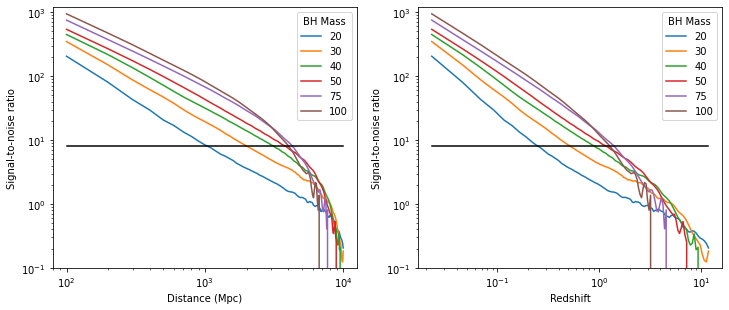
\includegraphics[width=5.25in]{SNR7.png}}
    \caption{\label{fig:massdistance} SNR of aLIGO at design sensitivity; black holes are assumed to be the same mass and equal to the template masses}
\end{figure}

As expected, there is almost a direct inverse relation between distance and SNR. However, this relation falls off at large distances, corresponding to high redshifts. This is particularly true for signals from larger black hole masses, which are of lower frequency and are therefore impacted more heavily at high redshifts due to the low frequency cutoff of 20 Hz. \\

Figure \ref{fig:massdistance} suggests that there is a threshold dependent on distance/redshift and SNR at which waveforms cannot be detected. From the redshift-SNR graph, the minimum SNR seems to be inversely proportional to the maximum redshift. 

\subsection{Imprecise Template Masses}

\begin{figure}[!htb]
    \center{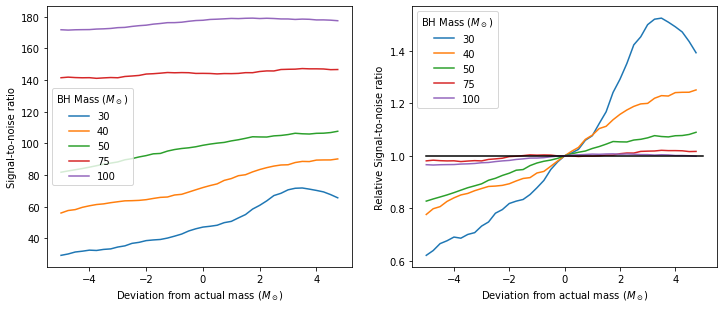
\includegraphics[width=5.25in]{SNR8.png}}
    \caption{\label{fig:imprecisemass} Absolute and relative SNR when using imprecise templates where both masses are the same; distance = 500 Mpc for all simulations}
\end{figure}

Similar to previous results, we see that the highest expectation value of SNR is achieved when the template waveform closely matches the parameters of the actual merger. However, as seen in Figure \ref{fig:imprecisemass} and \ref{fig:imprecisedistance}, the maximum is generally obtained when assuming the black holes are more massive than in actuality. This is likely because both redshift due to distance and larger masses causes the gravitational wave frequency to be lower. \\
 
From Figure \ref{fig:imprecisemass}, we observe that smaller deviations in mass lead to relatively larger changes in SNR for smaller masses. This is likely because the relative SNR is dependent on the percent change in mass, rather than the absolute difference; additionally, waveforms at higher masses are prone similar to each other.

\begin{figure}[!htb]
    \center{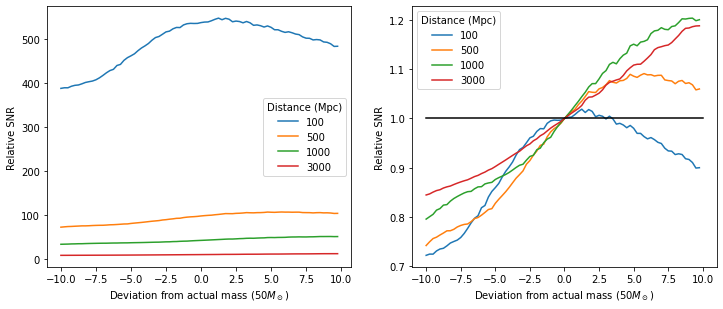
\includegraphics[width=5.25in]{SNR9.png}}
    \caption{\label{fig:imprecisedistance} Absolute and relative SNR when using imprecise templates where both masses are the same; mass = 50 $M_\odot$ for all simulations}
\end{figure}

From Figure \ref{fig:imprecisedistance}, we observe that the greater the distance of observation, the greater the mass correction needs to be to reach the maximum SNR. At a distance of $100$ Mpc, almost no correction is needed, as the redshift is negligible. 

\subsection{LIGO Sensitivity}

\begin{figure}[!htb]
    \centering
    \subfigure[]{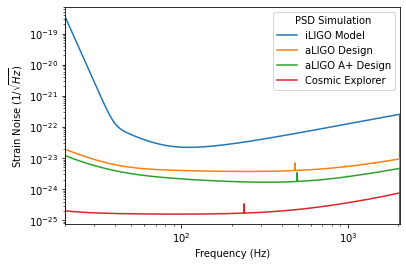
\includegraphics[width=0.49\textwidth]{SNR11.png}}
    \subfigure[]{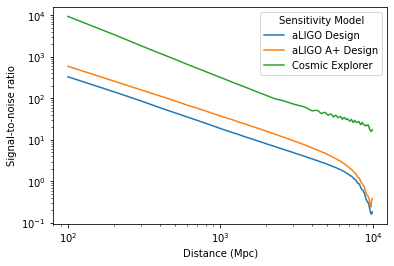
\includegraphics[width=0.49\textwidth]{SNR13.png}}
    \caption{\label{fig:psd} (a) Strain noise of different (modeled) LIGO sensitivities (b) SNR at different sensitivities, assuming both black holes are $30 M_\odot$ and identical to the template}
\end{figure}

We look at three sensitivity curves: the theoretical design sensitivity for aLIGO, A+ aLIGO, and Cosmic Explorer. The strain curves can be seen in Figure \ref{fig:psd}, in comparison to that of the design curve for iLIGO. These curves are only accurate above approximately $10$ Hz; at lower frequencies, it appears that the PSD is extrapolated arbitrarily. Figure \ref{fig:psd} therefore only depicts the curve between $20$ Hz and $2048$ Hz -- the cutoff lower bound frequency for generating waveforms for aLIGO and A+ will be $20$ Hz, and $10$ Hz for Cosmic Explorer. \\

A rough simulation of the SNR of the same black hole merger at different sensitivity models shows that aLIGO and A+ are relatively similar, as expected given their similar PSDs, while Cosmic Explorer vastly outperforms both. Even at large distances, the SNR of Cosmic Explorer remains above the (arbitrary) cutoff of 8, suggesting that the limiting factor in detecting black hole mergers will not be interference due to noise, but rather extreme redshifts that will essentially eradicate the entire length of the signal. 

\subsection{Varying Mass Ratio}

\begin{figure}[!htb]
    \center{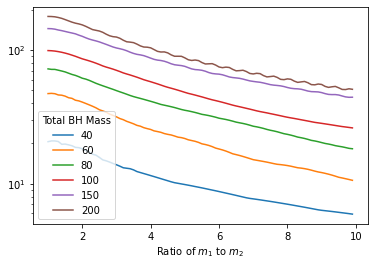
\includegraphics[width=3.5in]{SNR12.png}}
    \caption{\label{fig:ratiomass} SNR of aLIGO at design sensitivity with varying mass ratio given a constant total mass, assuming $m_1 \geq m_2$}
\end{figure}

Almost as important as the actual masses of each black hole in a merger is the ratio of masses of the two black holes, often denoted as the mass ratio $q \equiv m_1/m_2$. To avoid redundancy, we assume $m_1 \geq m_2$, so that $q \geq 1$ for all binaries. \\

We observe from Figure \ref{fig:ratiomass} that given a particular total mass, the greatest SNR is produced when the masses of the black holes are equal, and steadily decreases with more extreme mass ratios. This is in line with expectations as in a binary system with a highly skewed mass distribution, the binary acts similar to an orbital system in which only the smaller mass moves appreciably and therefore produces gravitational waves. Of course, the SNR is greater for larger total masses as well. 

\subsection{Maximum Redshift Distance}

The Schwarzchild metric for spacetime is 
\begin{equation}
    ds^2 = -(1-\frac{2M}{r}) dt^2 + (1 - \frac{2M}{r})^{-1} dr^2 + r^2 (d \theta^2 + \sin^2 \theta d\phi^2)
\end{equation}
This can be translated to Eddington-Finkelstein coordinates with the transformation 
\begin{equation}
    t = \nu - r - 2M \log \abs{\frac{r}{2M}-1}
\end{equation}
which results in the metric
\begin{equation}
    ds^2 = -(1-\frac{2M}{r}) d\nu^2 + 2 d \nu \; dr + r^2 (d\theta^2 + \sin^2 \theta d\phi^2)
\end{equation}
All light rays traveling in spacetime obey the formula $ds^2=0$. Looking specifically at radial light rays, characterized by $d\theta = d\phi = 0$, we arrive at the equation 
\begin{equation}
    ds^2 = -(1-\frac{2M}{r}) d\nu^2 + 2 d\nu \; dr = 0
\end{equation}
Dividing by $d \nu$ and solving for $d\nu/dr$, we find that there are two solutions: 
\begin{equation}
    \nu = \text{constant} \quad \text{or} \quad \nu - 2\Big(r + 2M \log \abs{\frac{r}{2M}-1}\Big) = \text{constant}
\end{equation}
The first solution corresponds to ingoing light rays, as from Eq. (2) if $\nu$ is constant, then $r$ must decrease as $t$ increases. The second solution describes ingoing rays for $r<2M$ and outgoing rays for $r>2M$. From this, we see that all light rays inside a sphere of radius $2M$ are ingoing -- therefore, the Schwarzchild radius, or the event horizon, is defined as 
\begin{equation}
    R = \frac{2GM}{c^2}
\end{equation}

Using this result, we can estimate the maximum frequency at which two black holes will orbit each other. As relativistic effects only significantly affect the inspiral for the last two or three orbits, we can use a Newtonian approximation. Kepler's Third Law states that 
\begin{equation}
    T^2 = \frac{4\pi^2}{GM}R^3
\end{equation}
If we suppose that the black holes are spheres with radius equal to its Schwarzchild radius, then it follows that the maximum frequency of orbit will occur when the black holes ``touch" each other; this will be the point at which they become inseparable. Therefore, 
\begin{equation}
    T^2 = \frac{4\pi^2}{GM} \Big( \frac{2Gm_1}{c^2} + \frac{2Gm_2}{c^2} \Big)^3 = \frac{32\pi^2 G^2 M^2}{c^6}
\end{equation}
It follows that the maximum frequency of orbit is 
\begin{equation}
    f_{\text{max}} = \frac{1}{T} = \frac{c^3}{\sqrt{32} \pi GM}
\end{equation}
If we suppose that a typical black hole merger has $M = 50 M_\odot$, then we find that 
\begin{equation}
    f_\text{max} = \frac{(2.998\times 10^8)^3}{\sqrt{32} \pi (6.674 \times 10^{-11}) (50) (1.988 \times 10^{30})} = 229 \text{ Hz}
\end{equation}
Therefore, the maximum redshift at which such a merger will produce potentially detectable gravitational waves, given a cutoff threshold of $20$ Hz, is 
\begin{equation}
    z_\text{max} = f_\text{max} / f_\text{low} = 229 / 20 \approx 11.4
\end{equation}
This corresponds to a comoving distance of approximately $10$ Mpc, which although is much further than what aLIGO design sensitivity could reasonably detect, falls within the potential detection radius of Cosmic Explorer. As seen in Figure \ref{fig:maxdistance}, this issue is much more pressing for extremely large mergers; however, the issue can be somewhat alleviated by lowering the cutoff frequency. 

\begin{figure}[!htb]
    \center{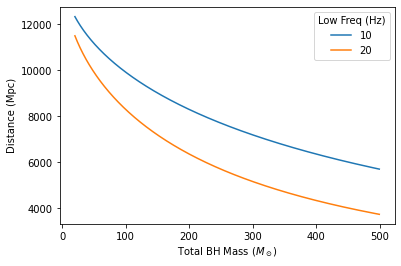
\includegraphics[width=3.5in]{SNR14.png}}
    \caption{\label{fig:maxdistance} Maximum distance of observation of a black hole merger given the total mass of both black holes}
\end{figure}

\end{document}

\begin{figure}[!htb]
    \center{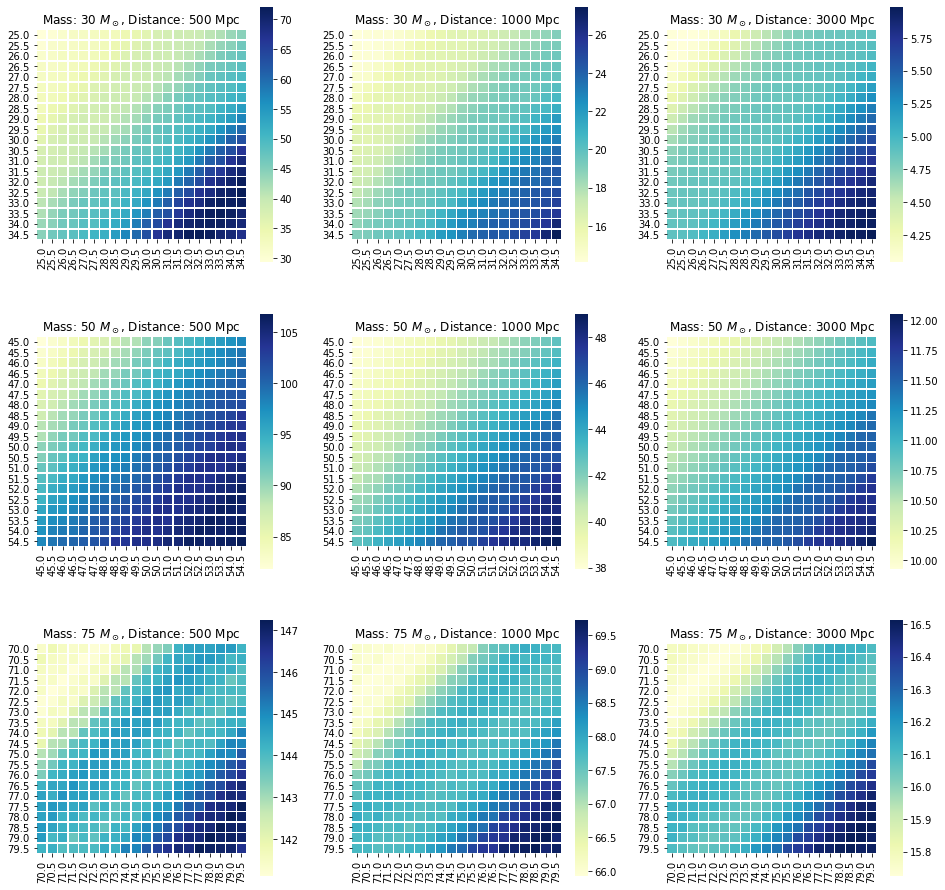
\includegraphics[width=\textwidth]{SNR10.png}}
    \caption{\label{fig:impreciseheatmap} Absolute SNR when using imprecise templates; actual mass of both black holes and distance of observation noted in title}
\end{figure}